
%%% outline
%-------------------------------------------------------------------------
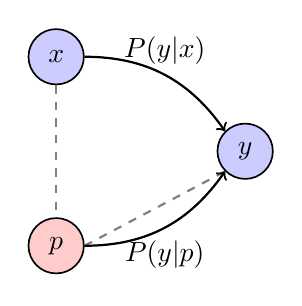
\begin{tikzpicture}

\node[draw,circle,inner sep=2pt,minimum size=2em,fill=blue!20,line width=0.6pt] (x) at (0,0) {$\seq{x}$};

\node[draw,circle,inner sep=2pt,minimum size=2em,fill=red!20,line width=0.6pt] (p) at (0,-2.4) {$\seq{p}$};

\node[draw,circle,inner sep=2pt,minimum size=2em,fill=blue!20,line width=0.6pt] (y) at (2.4,-1.2) {$\seq{y}$};

\draw[-,dashed,thick,black!50] (x.-90) -- (p.90);
\draw[-,dashed,thick,black!50] (p.0) -- (y.-135);
\draw[->,out=0,in=125,thick] (x.0) to node[above]{$\funp{P}(\seq{y}|\seq{x})$}(y.135);
\draw[->,out=0,in=-125,thick] (p.0) to node[below,yshift=-0.1em]{$\funp{P}(\seq{y}|\seq{p})$}(y.-135);

\end{tikzpicture}




